\documentclass[a4paper,12pt]{article}
\usepackage{graphicx}
\usepackage{amsmath}
\usepackage{amsthm}
\usepackage{amssymb}
\usepackage{algorithm}
\usepackage{algorithmic}
\usepackage{algpseudocode}
\usepackage{polski}
\usepackage[utf8]{inputenc}

\theoremstyle{definition}
\newtheorem{lemma}{Lemma}[section]

\DeclareMathOperator{\SA}{SA}
\DeclareMathOperator{\LCP}{LCP}
\DeclareMathOperator{\LPF}{LPF}

\title{A simple algorithm for Lempel-Ziv factorization}
\author{VM}

\begin{document}

\maketitle

Faktoryzacja Lempel-Ziv'a dla słowa $w$ jest takim rozkładem $u_0 u_1 ... u_k = w$,
 że każde $u_i$, za wyjątkiem możliwie ostatniego,
 jest albo najdłużsym prefiksem $u_i u_{i + 1} ... u_k$ i występuje jako podsłowo w $u_0 u_1 ... u_i$,
 ale nie tylko jako sufiks,
 albo jest pojedynczym symbolem, gdy takiego prefiksu nie ma.

Authorzy proponują algorytm pozwalający obliczać faktoryzację w czasie liniowym i pamięci $o(n)$.
Jeszcze poprzedni wynik tych samych autorów osiągał liniowy czas i pamięć,
 natomiast różnica pomiędzy dużym $O(n)$ tamtego algorytmu, i małym $o(n)$ dzisiejszego, jest na tyle istotna,
 że nowy algorytm został opublikowany.

Algorytm ten, tak jak i poprzedni, korzysta z tablicy Longest Previous Factor.
Aby zrozumieć co to jest, weźmy dowolne słowo $m$.
Aby $m$ było najdłużsym czynnikiem poprzednim,
 musi ono być najdłużsym podsłowem słowa $w[1..i + |m| - 1]$ spośród wszystkich możliwych prefiksów $w[i..n]$.
Wtedy jego długość będzie występować w tablicy LPF na pozycji $i$-tej.

Gdy już posiadamy tablicę LPF, wyznaczanie faktoryzacji nie jest trudne.
Łatwo zauważyć, że ``najdłuższy poprzedni czynnik'', to prawie dokładnie taki czynnik jakiego potrzebujemy do faktoryzacji.
Wystarczy zatem przejść po tablicy LPF zwracając kolejne czynniki,
 pomijając przy tym czynniki pośrednie, występujące pomiędzy tymi z faktoryzacji,
 oraz zamieniając wszystkie zera na jedynki w tablicy LPF, ponieważ faktoryzacja nie zawiera słów pustych.
\textbf{Algorithm 1} jest implementacją powyższego rozumowania.

\begin{algorithm}
\caption{lempel\_ziv\_factorization}
\begin{algorithmic}
\REQUIRE LPF, n
\ENSURE LZ
\STATE LZ $\gets [\;]$
\STATE pos $\gets$ 1
\WHILE{pos $\leq$ n}
\STATE push(max(1, LPF[pos]), LZ)
\STATE pos $\gets$ pos + max(1, LPF[pos])
\ENDWHILE
\end{algorithmic}
\end{algorithm}

Pozostaje wyznaczenie LPF. Do tego korzystamy z tablic SA, i LCP --
 z uporządkowanej tablicy sufiksów i tablicy najdłuższych prefiksów między nimi.
Nie będziemy projektować algorytmów do policzenia tych dwóch tablic,
 gdyż wiele takich istnieje.

\pagebreak

W szczególności, do policzenia tablicy SA proponowano jest użyć którykolwiek z poniższych algorytmów:
\begin{enumerate}
\item ``Simple linear work suffix array construction'' autorów J. Kärkkäinen i P. Sanders,
\item ``Linear-time longest-common-prefix computation in suffix arrays and its applications'' autorów T. Kasai, G. Lee, H. Arimura i S. Arikawa,
\item i ``Constructing suffix arrays in linear time'' autorów D.K. Kim, J.S. Sim, H. Park i K.Park,
\end{enumerate}
pamięciowa złożoność których jest usprawniona w pracy ``Space efficient linear time construction of suffix arrays'' autorstwa P. Ko i S. Aluru.

W przypadku LCP, algorytm z pracy ``Two space-saving tricks for linear-time LCP computation'' autora G. Manzini,
 też jest wystarczająco dobry aby nie wpłynąć na złożoność algorytmu LPF.

Zanim przejdziemy do właściwego obliczania LPF, zauważmy kilka własności związanych z jej wartościami.

\begin{lemma}

Wartości tablicy LPF są największymi wpsólnymi prefiksami między elementami tablicy SA.

\begin{proof}

Niech $w$ będzie słowem i $\SA_{i}$ będą kolejnymi tablicami prefiksów słowa $w$, uzupełnione o -1 na końcu.
Czyli $\SA_{i} = [ \SA[k] : \SA[k] \leq i ] \cup [-1]$.
Weźmy dowolne $i$, oraz indeks $x$ którego wartość jest maksymalna w tablicy $\SA_{i}$,
 czyli $x$ = $\max\limits_{y} \{ x : \SA_{i}[x] = y \}$.
Zauważmy, że dla takiego sufiksu $w[x .. n]$, odpowiedni najdłuższy czynnik poprzedni (w sensie definicji LPF)
 jest największym wspólnym prefiksem tego sufiksu z poprzednim lub z kolejnym sufiksem w tablicy SA.
Jest tak dlatego, że to te sufiksy są najbliżej sufiksu $w[x .. n]$, zatem mają najdłuższy wspólny z nim prefix.

\end{proof}
\end{lemma}

\begin{lemma}

Tablica LPF jest permutacją tablicy LCP.

\begin{proof}

Ponieważ największe wspólne prefiksy pomiędzy sufiksami $\SA_{n}$ to jest po prostu tablica LCP,
 wystarczy pokazać, że przejście od $\SA_{i}$ do $\SA_{i - 1}$ zawiera równoważne przejście w tablicy LCP.
Czyli, gdy $\SA_{i}$ jest nadzbiorem $\SA_{i - 1}$, to $\LCP_{i}$ też jest nadzbiorem $\LCP_{i - 1}$.
Zauważmy, że najdłuższy wspólny prefiks między eleementem $i$-tym i $(i + 2)$-ym jest mniejszy prefiks między $i$-tym i $(i + 1)$-ym a $(i + 1)$-ym i $(i + 2)$-im.
Zatem przejście definiujemy tak, że dla największego elementu w $\SA_{i}$, odpowiednie wartości $\LCP$ dla jego następnika
 to minimum wartości następnika i poprzednika maksymalnego elementu w $\LCP$, natomiast wszystkie inne wartości pozostają bez zmian.

\end{proof}
\end{lemma}

Mając na uwadzę takie własności, wystarczy przejść po tablicy $\SA$ w odpowiedniej kolejności 
 i aktualizować najdłuższe wspólne prefiksy w trakcie.

Aby zobaczyć jak dokładnie bedzie zmieniać się tablica sufiksów i tablica najdłuższych prefiksów,
 przydatne jest przedstawić ten proces w postaci grafu.

\begin{figure}[h!]
  \center
  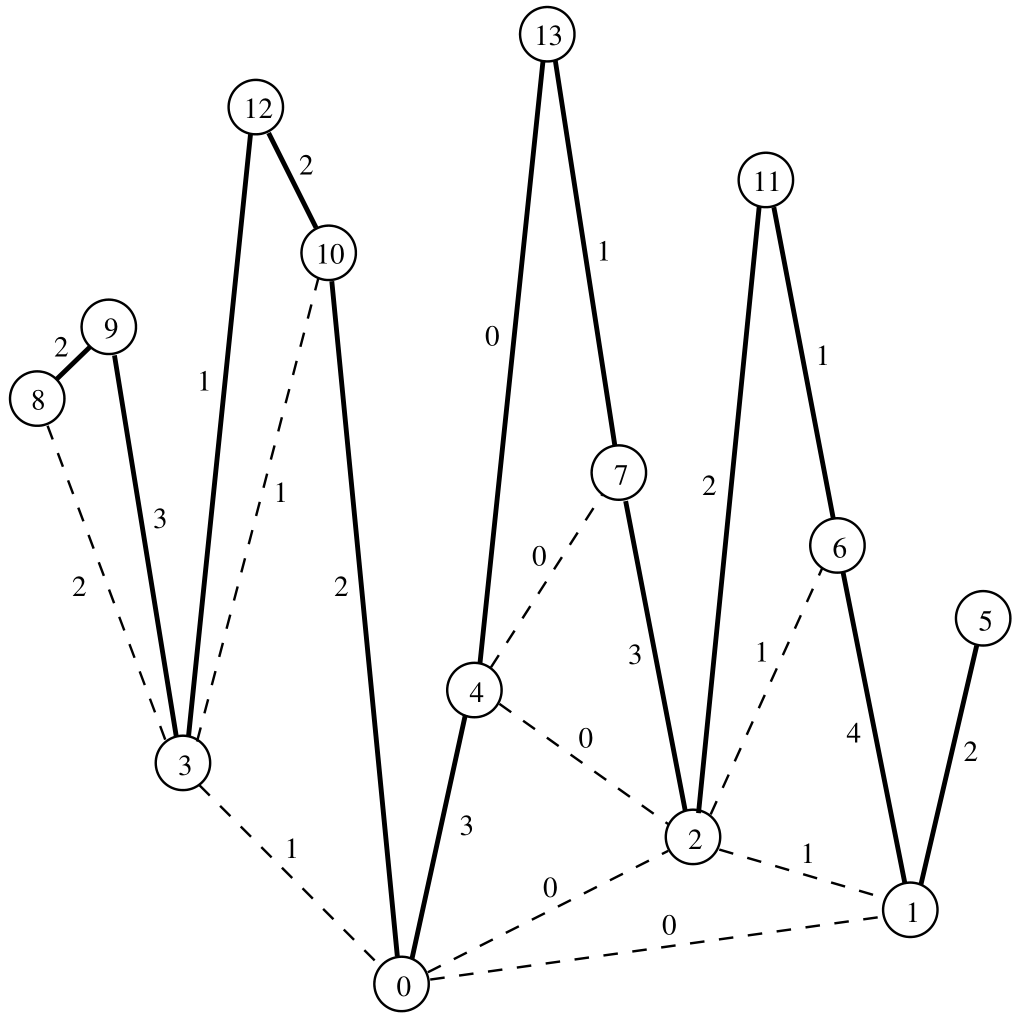
\includegraphics[width=0.6\linewidth]{graph}
  \caption{Graf ilustrujący zmieniający się stan w algorytmie LPF gdy słowo $abbaabbbaaabab$ jest na wejściu.}
\end{figure}

\pagebreak

Rysunek 1 należy odczytywać w następujący sposób:
\begin{itemize}
\item wartości w wieszchołkach to są kolejne wartości z tablicy $\SA$,
\item wartości przy krawędziach zwykłych to są wartości z tablicy $\LCP$,
\item wartości przy krawędziach przerywanych to są wartości tablic $\LCP_{i}$.
\end{itemize}

Algorytm obliczający LPF będzie iterować tablicę $\SA$ od lewej do prawej.
Trzy przypadki są do rozważenia:

\begin{enumerate}
\item[(1)] $\SA[i - 1] < \SA[i] > \SA[i + 1]$, czyli przypadek lokalnego maksimum.
  Ustawiamy $\LPF[\SA[i]] = \max(\LCP[i], \LCP[i + 1])$, oraz
  tworzymy nową krawędź zastępującą $\LCP[i], \LCP[i + 1]$ o wadze $\min(\LCP[i], \LCP[i + 1])$.
\item[(2)] $\SA[i - 1] < \SA[i] < \SA[i + 1] \land \LCP[i] \geq \LCP[i + 1]$.
  Analogicznie do przypadku (1).
\item[(3)] $\SA[i - 1] > \SA[i] > \SA[i + 1] \land \LCP[i] \leq \LCP[i + 1]$.
  Ponieważ my idziemy od lewej do prawej, to przypadek (1) zapobiega występowaniu takiego scenariusza.
\end{enumerate}

Algorytm będzie próbował stosować reguły (1) i (2) na każdym kroku iteracji.
Aby zachować odpowiednią kolejność, utrzymywany będzie stos indeksów do tablic $\SA$ i $\LCP$.
W ten sposób otrzymujemy \textbf{Algorithm 2}.

\begin{algorithm}
\caption{compute\_lpf}
\begin{algorithmic}
\REQUIRE SA, LCP, n
\ENSURE LPF
\STATE SA[n + 1] $\gets [\;]$ -1
\STATE LCP[n + 1] $\gets [\;]$ 0
\STATE push(1, L)
\FOR{i = 1 $\TO$ n + 1}
\WHILE{L $\neq$ $\emptyset$ $\land$ \\
       \qquad (SA[i] $<$ SA[TOP(L)] $\lor$ \\
       \qquad (SA[i] $>$ SA[TOP(L)] $\land$ LCP[i] $\leq$ LCP[TOP(L)]))}

\IF{$SA[i] < SA[TOP(L)]$}
LOL
\ENDIF

\STATE KEK
\ENDWHILE
\STATE push(max(1, LPF[pos]), LZ)
\STATE pos $\gets$ pos + max(1, LPF[pos])
\ENDFOR
\end{algorithmic}
\end{algorithm}

\end{document}
